\documentclass[aps,pre,12pt,preprint,%
	onecolumn,showpacs,showkeys,nofootinbib]{revtex4-1}
%Chinese
	\usepackage[UTF8,fontset=fandol]{ctex}
	\xeCJKsetup{underdot = {
		boxdepth=0pt, format=\huge, depth=.4em
	}}
%	\usepackage[datesep=/]{datetime2} % Use default
	\DeclareTextFontCommand{\textbf}{\sffamily}
%Presenting
	\usepackage[table]{xcolor}
	\usepackage{graphicx}
	\usepackage[space]{grffile}
	\usepackage[font=small,format=plain,%
		labelfont=bf,textfont=it,%
		singlelinecheck=false]{caption}
	\usepackage[above]{placeins}
%	\usepackage{float} % Cause trouble for table footnotes
	\usepackage{wrapfig}
	\usepackage{tabularx,array,booktabs,multirow,bigstrut}
	\newcolumntype{C}[1]{>{\hsize=#1\hsize%
		\centering\arraybackslash}X}
	\newcommand{\minitab}[2][l]{%
		\begin{tabular}{#1}#2\end{tabular}}
	\usepackage{setspace,dcolumn}
	\usepackage{subfig}
	\usepackage{psfrag,epsfig}
%MathSetting
	\let\latexointop\ointop
	\usepackage{amsmath,bm,amssymb,esint,extarrows}
	\usepackage{upgreek,textcomp,mathrsfs}
	\usepackage[only,sslash]{stmaryrd}
	\usepackage{nicefrac,eqnarray}
%	\usepackage{amsthm} % Enable when necessary
%	\usepackage[mathscr]{eucal} % Enable when necessary
	\usepackage{mathtools,physics,siunitx}
	\usepackage{stackengine,varwidth}
	\usepackage{tikz}
	\usepackage{resizegather,empheq}
	\usetagform{default}
	\usepackage{calligra,fourier-orns}
	% Keep \oint unchanged by esint
	\let\ointop\undefined
	\let\ointop\latexointop
	% Define a scriptr 
	\DeclareMathAlphabet{\mathcalligra}{T1}{calligra}{m}{n}
	\DeclareFontShape{T1}{calligra}{m}{n}{<->s*[2.2]callig15}{}
	\newcommand{\scriptr}{\mathcalligra{r}\,}
	\newcommand{\rvector}{\pmb{\mathcalligra{r}}\,}
	% Useful shorthand
	\DeclarePairedDelimiter\ave{\langle}{\rangle}
	\newcommand\inlineeqno{\stepcounter{equation}\ (\theequation)}
	\newcommand{\sinc}{\operatorname{sinc}}
	\newcommand{\mbb}[1]{\mathbb{#1}}
	\newcommand{\mrm}[1]{\mathrm{#1}}
	\newcommand{\mcal}[1]{\mathcal{#1}}
	\newcommand{\tup}[1]{\textup{#1}}
	% Scaling and positioning
	\newcommand\scalemath[2]{\scalebox{#1}{\mbox{\ensuremath{\displaystyle #2}}}}
	\newcommand\raisemath[2]{\raisebox{#1\depth}{${#2}$}}
	\empheqset{box=\nicebox}
	% Presenting
	\newcommand*\nicebox[1]{\fbox{\hspace{1em}\addstackgap[5pt]{#1}\hspace{1em}}}
	\sisetup{%
		redefine-symbols=false,%
		separate-uncertainty=true,%
		range-phrase=\,\textasciitilde\,,%
		arc-separator = \,}
	\allowdisplaybreaks[2]
%ParagraphSetting
	\setlength{\parskip}{.3\baselineskip}
	\usepackage[defaultlines=2,all]{nowidow}
	\postdisplaypenalty=50
%PageSetting
	\usepackage{titlesec}
	\titleformat*{\section}{\large\bfseries}
	\usepackage[colorlinks=true,linkcolor=blue]{hyperref}
	\newcommand{\texstringonly}[1]{%
		\texorpdfstring{#1}{}}
	\usepackage[vmargin={3.5cm,4cm},hmargin=3cm,%
		footnotesep=\baselineskip]{geometry}
%	\usepackage[bottom]{footmisc} % Cause trouble for table footnotes
	\usepackage{changepage}
	% Autoref names
	\renewcommand{\tableautorefname}{\tablename}
	\renewcommand{\figureautorefname}{\figurename}
	% List settings
	\usepackage{enumitem}
	\setlist{itemsep=0pt,topsep=0pt,labelindent=\parindent,leftmargin=0pt,itemindent=*}
	% Some redefined lengths
	\setlength{\headsep}{1.6\baselineskip}
%	\setlength{\footnotesep}{3\parskip} % Use when necessary
	% Header
	\usepackage{fancyhdr,lastpage}
	\pagestyle{fancy}
%	\fancyhf{} % Clear default settings; disabled for now
	\cfoot{--\ \thepage\,/\,\pageref{LastPage} \ --}
	\setlength{\footskip}{2\baselineskip}
	\renewcommand{\headrulewidth}{0.1pt}
	\renewcommand{\headrule}{
		\ifnum\value{page}=1\relax\else
			\vbox to 2pt{
			\hbox to \headwidth{\dotfill}\vss}
		\fi}
	\fancypagestyle{titlepagestyle}{%
		\fancyhead{}
		\chead{
			\vspace{2.5\baselineskip}
			
\includegraphics[width=.75\linewidth]{../PKUPhy}}
	}
	% Separator
	\newcommand{\newparagraph}{\pagebreak[3]\noindent%
		\hfil
		~\raisebox{-4pt}[10pt][10pt]{\decofourright~~~~~~~~\decofourleft}~ %
		\par
	}
%	% Background % Use when necessary
%	\usepackage{background} %Waterstamp package
%	\SetBgContents{...的实验报告} %Waterstamp to prevent copying
%	\SetBgScale{5} %Waterstamp setting
	% Essay format
	\renewcommand\appendixname{附录}
	\renewcommand\abstractname{}%摘要
	\renewcommand\tablename{表}
	\renewcommand\figurename{图}
	\renewcommand\refname{参考文献}
	\makeatletter
	\def\@pacs@name{\songti\zihao{-4}{\bf PACS码:}}
	\def\@keys@name{\songti\zihao{-4}{\bf 关键词:}}
	\def\Dated@name{日期:}
	\def\Received@name{\zihao{-5}{接收} }
	\def\Revised@name{\zihao{-5}{修订} }
	\def\Accepted@name{\zihao{-5}{采纳} }
	\def\Published@name{\zihao{-5}{发表} }
	\makeatother
	\linespread{1.5}
	\renewcommand{\labelenumi}{\alph{enumi}.}
	\leftmargini=20mm
	\newcommand{\supercite}[1]{\textsuperscript{\,%
		[\citenum{#1}]}}
	\let\fancycite\cite
	\renewcommand{\cite}[1]{\textup{\fancycite{#1}}}
	% Math line spacing
	\newlength{\djot}
	\setlength{\djot}{\jot}
	\newcommand{\restorejot}{\setlength{\jot}{\djot}}

\usepackage{transparent}
%Miscellaneous
%	\newcommand{\tabindent}{\hspace{2em}}
%FourierTransform
	\newcommand{\fourierf}{\mathscr F}
\begin{document}
%Basic Data
	\title{%
	\texstringonly{\hfil\\[2\baselineskip]}
	\sf\LARGE%
		利用扫描隧穿显微镜获得原子分辨像%
	\texstringonly{\vspace{3ex}}}
	\author{\fangsong\large%
		Bryan%
	\vspace{2mm}}
	\affiliation{\it%
		北京大学物理学院~~学号:\normalfont 1500000000\,}
	\date{\today}
	\keywords{隧穿效应,扫描隧穿显微镜(STM),高定向热解石墨(HOPG),\\
		\hphantom{关键词:}原子分辨图像,压电陶瓷,压电系数}
	\email{guesswhat@email.addr;}

\begin{abstract}
\vspace{10mm}
\begin{spacing}{1.5}\normalsize
\setlength{\parskip}{.3\baselineskip}
%	200—300字,
%	说明用什么方法做了什么事,
%	由此得到什么结果和结论,
%	有何意义.
%	不用缩略词,不用第一人称.
%
	本实验使用扫描隧穿显微镜(Scanning tunneling microscope, STM)获得了样品表面的原子分辨像,从而直观地验证量子隧穿效应;同时,总结了隧穿电流的变化规律,并在此基础上探讨了隧穿显微技术的应用。

	实验中观察的样品为结构已知的高定向热解石墨(Highly oriented pyrolytic graphite, HOGP);本实验通过比较STM所成图像与样品实际结构,粗略地校准了STM的探针控制系统,从而使其能较为精确地获得结构未知样品的原子分辨像。
\end{spacing}
\end{abstract}

\maketitle
\thispagestyle{titlepagestyle}
%
%	\item 课程实验报告应假定读者既不是已知全部实验细节的指导教师,也不是缺少专业知识的公众,而是同领域的实验研究者,或审稿人. 不能要求读者要在读过课程讲义后才能读懂课程实验报告.
%	\item 公式、图和表要分别用阿拉伯数字编列序号. 公式和图表要达到可发表的质量.
%	\item 凡不是自己独立思考得到的内容都应该引参考文献. 不能大段引用同一参考文献. 对复杂问题,应该优先考虑引用参考文献得到结果. 对简单一些的问题才鼓励独立思考.
%	\item 较长的推导和说明可以作为附件提交,不占用报告篇幅.
%	\item 思考题不是报告的组成部分. 应另起一页附在报告的最后.
\section{引言}
%%	研究论文引言一般包含以下内容:
%%	(1)所研究领域背景和现状;
%%	(2)有待研究的问题;
%%	(3)本研究的目的、主要内容和结果;
%%	(4)结果的意义.\par
%%	在写实验报告的引言时,同学可以假想自己是第一个做类似研究的人.\par
%%	引言一定要切合报告正文,不能漫无目的地介绍背景. 要快速地将读者引导到报告主题上,并作较深入的讨论.\par
%%	引言篇幅可以在较大范围内变化,但最长不应超过报告文字篇幅的1/3.\par
%%	引言撰写可以参考实验讲义,可以复述,但不能复制讲义上的任何一句话.\par
%%%%%%%%%%%%%%%%%%%%%%%%%%%%%%%
	在一定条件下,微观粒子能够穿入或穿越高于其总能量的势垒;这一极端非经典的现象称为隧穿效应(Quantum tunneling)。
	
	早在1901年,Robert Francis Earhart在研究气体放电时发现了异常的电导,这可能是隧穿效应的首个实验迹象\supercite{tunnelOrigin}。在此后的20余年间,实验中多次观测到隧穿电流,但并没有成熟的理论解释;事实上,由于观测到的隧穿电流十分微弱(在 \SI{10}{\pA} 量级),这一效应并没有得到充分的重视\supercite{mohsen2003quantum}。
	
	1926年,薛定谔发表了波动方程,严谨的量子力学体系得以建立;在此基础上,1927年洪德(Friedrich Hund)首次从理论上发现了隧穿效应,他和伽莫夫(George Gamow)等人将其应用于原子核衰变的研究中;但当时人们并没有意识到,这一现象不仅局限于核物理范畴,还能有可直接观测的效应\supercite{mohsen2003quantum}。
	
	隧穿在量子体系中的普遍存在是波恩(Max Born)首先提出的;在随后关于半导体的研究中,这一观点被充分证实,此后隧穿及其理论解释才被广泛地接受\supercite{mohsen2003quantum}。
	
	1981年,IBM苏黎世实验室的格尔德·宾宁(G.~Binging)和海因里希·罗雷尔(H.~Rohrer)首次成功利用隧穿效应获得了原子分辨像,发明了第一台扫描隧穿显微镜(STM, scanning tunneling microscope)。STM的工作强烈地依赖于精确到 \si{\angstrom} 量级的位置控制,这通过对压电陶瓷加压得以实现\supercite{binnig1982surface}。事实上,完全类似的想法曾由R.~Young等人在1970年代初期提出\supercite{young1972topografiner}, 但由于技术上的限制,他们未能得到出色的结果。1986年,STM获得诺贝尔物理学奖。
	
	本次实验中,我们力图采用完全类似的方法,重现宾宁和罗雷尔的实验;通过观测已知的材料——高定向热解石墨(HOPG, Highly oriented pyrolytic graphite),验证这一技术的有效性。此外,我们将考察压电材料在此实验中所起的关键作用,并检验本实验采用的陶瓷之压电特性。由于水平面上的精准定位对成像质量(防止畸变)尤为重要,我们将仅考察控制$x,y$位置的压电陶瓷,以此粗略地校准定位系统,为精准测定创造条件。
\section{理论}
	简单起见,考察一维定态薛定谔方程:
	\begin{equation}
		- \frac{\hbar^2}{2m} \dv[2]{\psi}{x}
			+ \pqty\big{V(x) - E}\,\psi(x) = 0
	\end{equation}
	以此描述针尖与样品之间的电子流。首先,对于不存在势垒的情况(\textit{可以想象针尖与样品表面以导电介质连通}),此时在一定的偏压下,稳恒电子流可由平面波函数描述:
	\begin{equation}
		\psi(x) \sim e^{ikx},\quad
		k = \frac{p}{\hbar} = \frac{\sqrt{2mE}}{\hbar}
	\end{equation}
	
	\begin{figure}[!h]
	\centering
	\vspace{-0.5\baselineskip}
	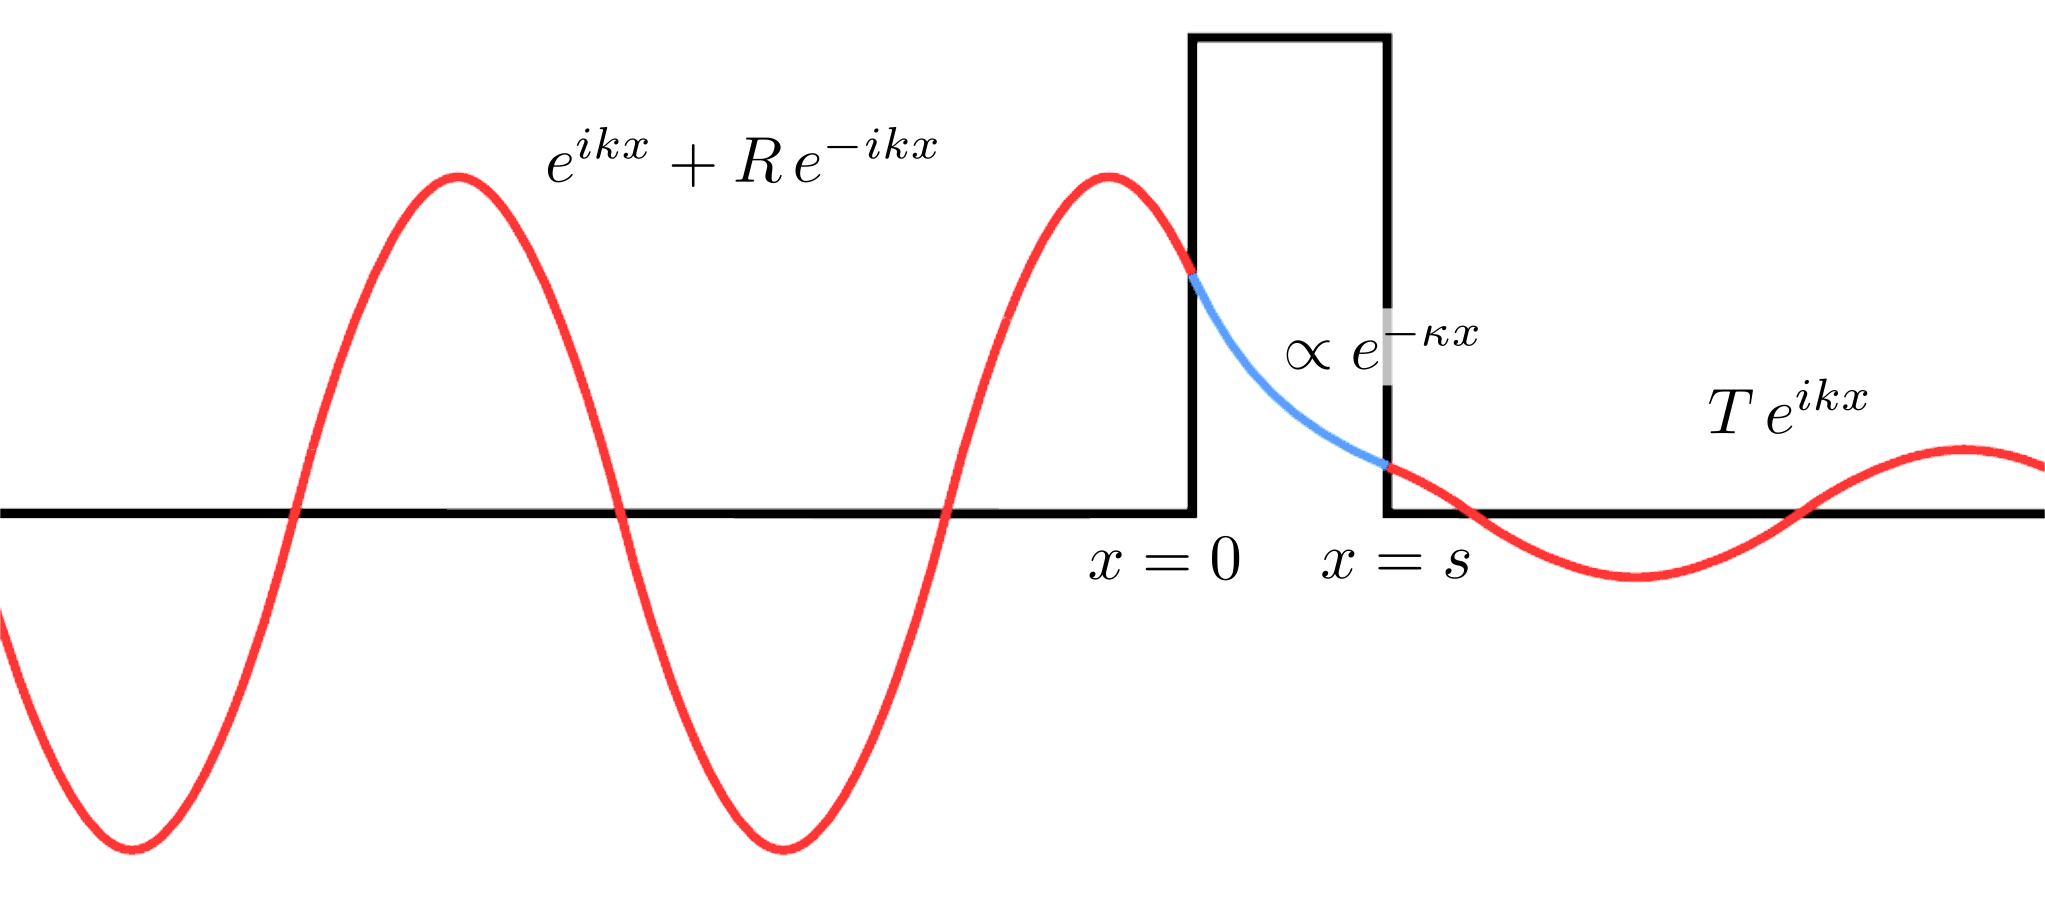
\includegraphics[width=.8\linewidth]{TunnelEffect.png}
	\caption[量子隧穿的一维描述]{量子隧穿的一维描述\footnote{%
			图像据网络资源修改得到:\par
			\noindent%\fontsize{9pt}{\parskip}%
			\url{https://en.wikipedia.org/wiki/File:TunnelEffektKling1.png}%
		},参考 \cite{griffiths2016introduction}. \\
		稳恒电子流由左向右入射方形势垒,透射波的振幅减小,频率$k$不变。
		\vspace{.5ex}
	}
	\label{fig:Tunnel1D}
	\end{figure}
	
	\vspace{1ex}
	若存在势垒,设其高度为$\phi$, 而针尖位于$x = 0$处,样品表面位于$x = s$处,则$V(x)$的分布可以粗略地表示为:
	\begin{equation}
		V(x) = \Bigg\lbrace\,
		\begin{aligned}
			\phi, \quad& 0 < x < s,\\
			0, \quad& x < 0 \ \textrm{or}\  x > s, 
		\end{aligned}
	\end{equation}
	如\autoref{fig:Tunnel1D} 所示,其中入射波、反射波、透射波均采用平面波近似:
	\begin{equation}
		\textit{入射:} e^{ikx},\quad
		\textit{反射:} R\,e^{-ikx},\quad
		\textit{透射:} T\,e^{ikx},
	\end{equation}
	
	求解薛定谔方程,我们发现,$0 < x < s$区域内的波函数并不为0, 而是具有指数衰减的形式:
	\begin{gather}
		\psi(x) \propto e^{-\kappa x},\quad 0 < x < s,\\
		\kappa = \frac{\sqrt{2m(\phi - E)}}{\hbar}
			\sim \frac{\sqrt{2m\phi}}{\hbar}
	\end{gather}
	这里采用了近似处理,假定势垒高度$\phi \gg E$. 进一步,由于电流$I$与电子透射率线性相关,求解得到:
	\begin{equation}
		\frac{I}{I_0} = \abs{T}^2
		\sim \frac{16E}{\phi} e^{-2\kappa s},\quad
		\kappa \sim \frac{\sqrt{2m\phi}}{\hbar}
	\end{equation}
	同样采用了近似条件$\phi \gg E$, 其中$I_0$为势垒为0时的电流大小。
	
	综上,我们得到了隧穿电流的估计式:
	\begin{equation}
		I \sim B\,e^{-2\kappa s},\quad
		\kappa \sim \frac{\sqrt{2m\phi}}{\hbar},\quad
		B \sim I_0 \frac{16E}{\phi}
		\label{eq:tunnelEq}
	\end{equation}
	针尖与样品之间所加的偏压$V_\textup{b}$越大,相应的$I_0, E$越大,隧穿电流越大;同时,势垒宽度$s$越大,隧穿电流越小,且为指数衰减。在控制真空度一定的情形下,可以假定势垒高度$\phi$基本恒定。
	
	工作状态下,本实验中的STM针尖与样品间距$s \sim \SI{1}{\nm} = \SI{10}{\angstrom}$, 电流改变一个量级对应的$\var{s} \sim \SI{0.1}{\nm} = \SI{1}{\angstrom}$, 正是原子间距的尺度\footnote{%
		参见 \cite{textbook}, p.~224. }。
	这自然导致了STM的高分辨率,同时也对装置的机械稳定性提出了很高的要求。
	
	此外,这也表明隧穿电流局域在针尖和样品原子间极端细长的范围内,此区域内上述一维模型基本成立;针尖附近隧穿电流的实际分布如\autoref{fig:Current2D} 所示。
	
	\begin{figure}[!h]
	\centering
	\vspace{-0.5\baselineskip}
	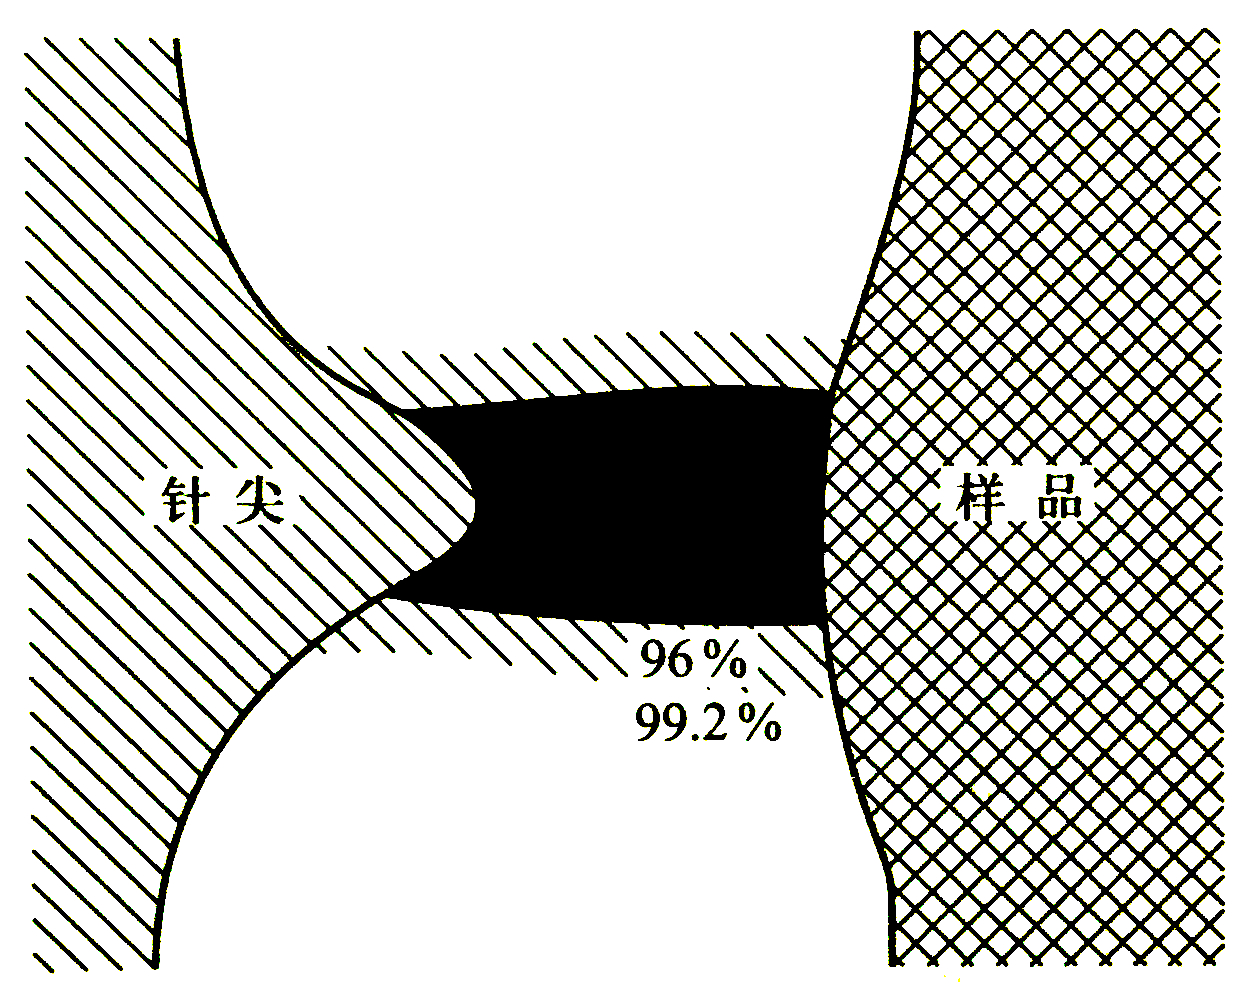
\includegraphics[width=.55\linewidth]{STMcurrentDist.jpg}
	\caption[隧穿电流的三维分布]{针尖附近隧穿电流的三维分布,
		通过更精细的理论计算得到,摘自 \cite{stmIBM}. \\
		百分比表明该区域电流占总电流的比例,\\
		可见隧穿电流局域在针尖和样品原子间极端细长的范围内。
		\vspace{.5ex}
	}
	\label{fig:Current2D}
	\end{figure}
\section{实验装置}
%%	在此部分需要将实验条件交待清楚到别人能重复你的实验结果的程度. 此外,还需表明你已尽了最大努力来提高实验精度和结果的可靠性. 简单的不确定度估计可以在此节给出,复杂一些的可以放到分析讨论部分.\par
%%	实验条件不仅是指直接影响实验结果的实验参量,而且还包括影响实验质量和可靠性的因素,如室温、空气湿度、基真空、原材料纯度等.\par
%%	作为教学实验报告,此节写详细一点没有坏处.\par
%%	成段有叙述,必要才分节。
%%%%%%%%%%%%%%%%%%%%%%%%%%%%%%%
	本实验采用由北大实创公司研制生产的DS-2000A型STM, 其原理与 \cite{binnig1982surface} 完全一致;核心部分的示意见\autoref{fig:stmSchematic}. 系统的控制和数据采集由两部分组成,分别是计算机自动化系统(以下简称PC)和实体的控制面板(由各类旋钮构成)。
	
	实验中,成像区域的精准定位通过压电陶瓷实现,其(\textit{在固定方向上的})外加电压$V$和实际伸长$l$之间有良好的线性关系:
	\begin{equation}
		l = c\,V,\quad c > 0
		\label{eq:piezoEq}
	\end{equation}
	这里的$c$称为压电系数。因此,实验中的坐标可相应地由$V_i,\,i=x,y,z$表示。
	
	我们采用\textit{恒电流模式}进行扫描成像。设定初始隧穿电流$I$, 当针尖移过样品崎岖不平的表面时,若检测到隧穿电流的微小变动$\var{I} > 0$, 则表明针尖与样品的距离$s$变小,即$\var{s} < 0$. $\var{I}$的值经过一定的放大增益,传入反馈电路;反馈电路立即减小$z$电压$V_z$, 使得压电陶瓷的$z$伸长$l_z$变小,从而针尖与样品重新远离,隧穿电流回复到初始值$I$。
	
	这一负反馈过程应当充分的灵敏、快速,使得扫描过程中$I,s$几乎不变,这样针尖划出的轨迹正是样品表面的形貌,如\autoref{fig:stmSchematic} 所示。记录相应的$(V_x,V_y,V_z)$值,便可在PC上重建样品表面的图像。
	
	\begin{figure}[!h]
	\centering
	\vspace{-0.5\baselineskip}
	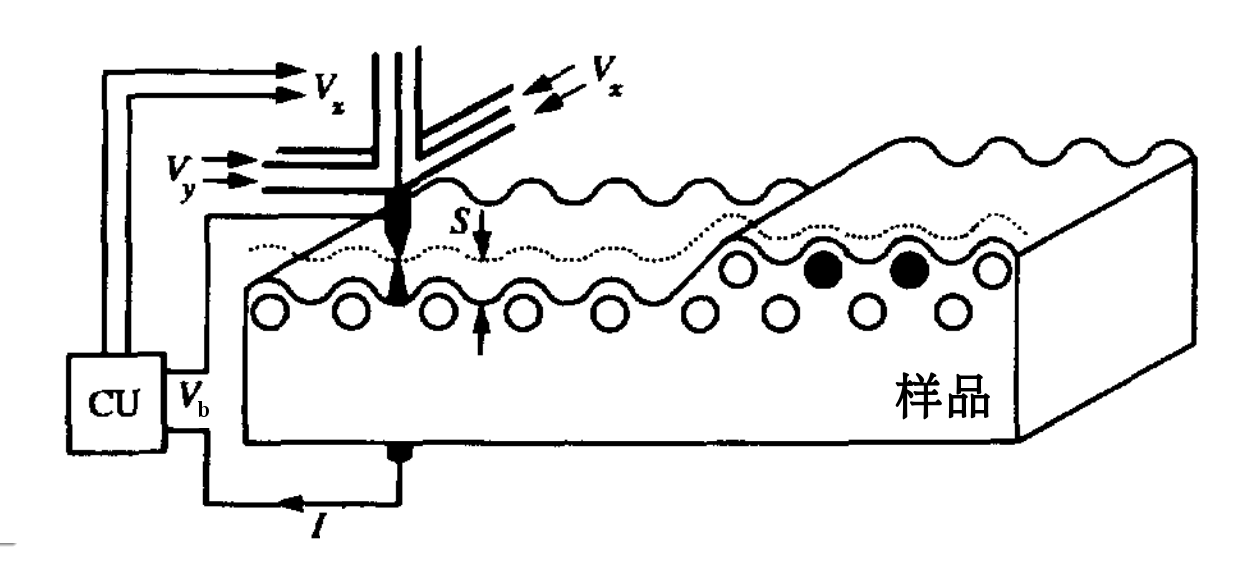
\includegraphics[width=.75\linewidth]{stmSchematic.png}
	\caption[STM原理]{\textup{STM}原理示意图,参考 \cite{stmIBM}. \\
		$V_x,V_y,V_z$表示加在压电陶瓷上的电压,分别控制针尖在$x,y,z$方向上的移动;\\
		在恒流模式下,$V_x,V_y$只是平凡的扫描电压;\\
		而$V_z$则接入反馈控制单元,使得隧穿电流$I$及间距$s$保持恒定。
		\vspace{.5ex}
	}
	\label{fig:stmSchematic}
	\end{figure}
	
	反馈过程具有一定的响应时间,因此横向的扫描不能太快,即扫描时间$T$不能太小,否则反馈电路无法跟进,导致成像不理想,甚至使针尖撞上样品损毁。
	
	\textbf{初始设置:}调节面板旋钮,设置$V_{x,y}$的起点(ORIGIN)为 \SI{0}{\volt}, 变化范围(RANGE)调至最大:\SI{200}{\volt}. 调整预期的隧穿电流$I \sim \SI{1}{\nA}$, 本次实验中的设定值为$I = \SI{1.13}{\nA}$. 
	
	此外,对于初始阶段大范围内的扫描,不需要太强的$z$信号输出;因此,暂且调整信号增益(Amplification, 以下简称Amp)旋钮至$\boxed{\times 20}$处。
	
	\textbf{自动进针:}由于压电陶瓷的伸长范围有限,首先应当使用\CJKunderdot{机械}粗逼近系统将针尖移近样品,直至隧穿发生。在PC上启动自动进针,系统监测到非零的隧穿电流后立即自动停止,并发出警报。
	
	此刻,间距$s$取临界值,隧穿效应恰能发生,仅有十分微弱的隧穿电流;但装载陶瓷和针尖的机械结构离样品还有一定距离。然而,此时$z$方向的负反馈电路已开始工作,故系统迅速增大$V_z$, 使得针尖与样品表面强行接近,直到隧穿电流达到预设值$I = \SI{1.13}{\A}$; 这时$z$陶瓷处于极致伸长的状态,面板上可以读出此时的$V_z$, 其值往往很大,在 \SIrange{100}{200}{\V} 以上。
	
	当前状态下,如果直接开始扫描,为了保证隧穿电流$I$恒定,反馈电路要求的$V_z$变化可能超过上限;而实际上,机械结构与样品的间距还充分地远,因此可以安全地手动调节粗逼近系统:在PC上控制单步进针,关注$V_z$示数,可见其逐步减小,直到它降至 \SI{90}{\V} 左右;这样便可充分利用$z$陶瓷的“量程”。
	
	此时,为确保安全,再单步退针20下;由于机械系统的回程差,$V_z$基本不变。至此,STM粗调完毕。在此基础上进行实验。
\section{结果与分析}
%	实验结果应尽量以图表的形式给出. 每一个图表都应该是完整的,即阅读图表时可以不必依赖正文.\par
%	依自己意愿,实验结果和对结果的分析讨论既可分为两节也可合在一节.\par
%	\begin{table}[h]
%	\caption{元件恒流大小,为什么要左对齐呢?奇怪。}
%	\small
%	\begin{tabularx}{.6\linewidth}{C{.3} C{1}}
%	\toprule
%	\midrule
%		元件\footnote{%
%			注释一个看看%
%		} & 恒流大小\footnote{%
%			再开一个!哈哈
%		} \\
%	\midrule
%		Pt  &
%			$\SI{1.00005}{\mA}
%				= \SI{100.005}{\mV} / \SI{100}{\ohm} $ \\
%	\midrule
%	\bottomrule
%	\end{tabularx}
%	\label{tab:ExTab}
%	\end{table}
%
%	每个图一般包含:图名、轴名、轴、刻度、标尺、数据点、曲线、图例、标注和图注等部分. 应尽量让读者不看正文就能基本理解图的含意.\par
%	逐点测量得到的函数关系要同时用表格和图给出. 需要作比较的多条曲线要画在同一图上.\par
%	为避免读者在图表和正文间反复跳跃阅读,在正文中也要对图表作必要的说明.\par
%
%	对于预料之外的实验结果,必须首先小心证明其可靠性.读者只有在相信你的实验结果时才愿意花时间看你的分析.\par
%	必须用文字归纳整理出正式的实验结果或结论.可信的实验结果是课程报告最重要的内容.作为一个实验物理工作者,分析解释出错并不丢脸,实验结果不被采信则是致命的.\par
%	教学实验的结论往往是预先知道的. 所以,教师更关心的是你的说理过程. 一般说来,单由课内实验的结果不足以能得到明确的结论. 此时,你可以引用他人的研究结果来帮助帮助自己的论证,但必须注明出处. \par
%	确实不能得到明确结论时,可以给出几种可能结论并指出可以再做哪些实验来帮助作进一步的判断.\par
%	总之,分析讨论部分要做到: 论据要valid,论证要reasonable,结论要convincing.\par
%%%%%%%%%%%%%%%%%%%%%%%%%%%%%%
\subsection{大范围扫描}
	首次扫描,在PC上设定偏置电压$V_\textup{b} = \SI{1000}{\mV}$, 扫描时间$T = \SI{2000}{\ms}$, 调整增益(Amp)旋钮至$\boxed{\times 20}$处。
	扫描时若发现信号过强被截断,可调节Offset旋钮,即调整电平零点,使得信号波形被完整地记录下来;最终结果如图 \ref{fig:firstTry-a} 所示。
	
	在此基础上,选取图像中的平坦区域,一步步缩小$x,y$扫描范围、调整扫描起点,以获得更加精细的扫描图像;可相应成比例地缩小扫描时间,以提升扫描效率。如此重复,直到达到原子分辨为止。仔细观察图 \ref{fig:firstTry-b}, 可以隐约看到斜向的条纹,这很可能是原子尺度的表面形貌。
	
	\begin{figure}[p]
	\centering
	\vspace{-1\baselineskip}
	\subfloat[大范围初始扫描]{\label{fig:firstTry-a}
		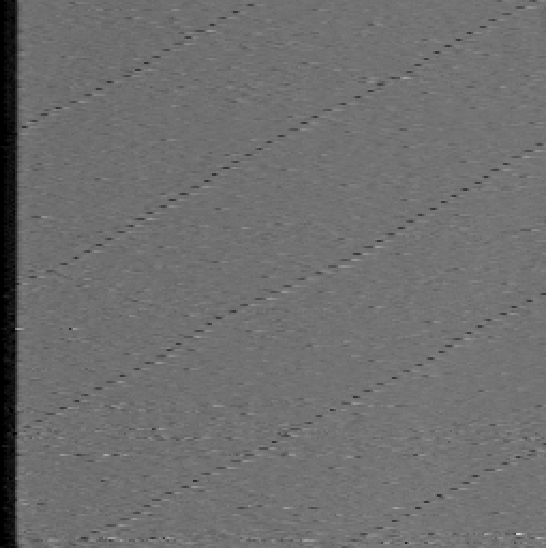
\includegraphics[width=.45\linewidth]{img/1404 - 初始扫描.png}}
	\quad
	\subfloat[出现原子分辨迹象]{\label{fig:firstTry-b}
		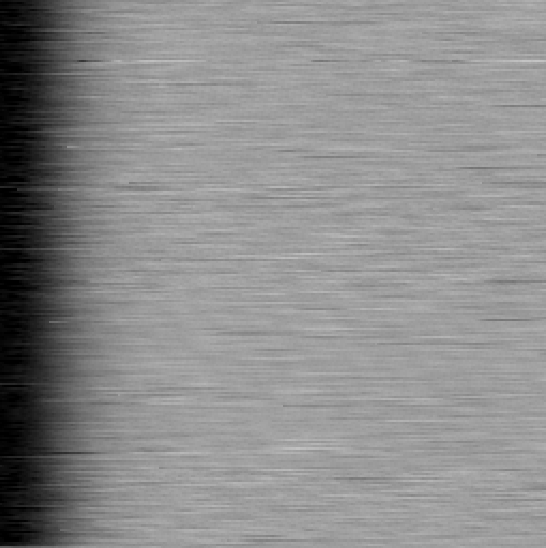
\includegraphics[width=.45\linewidth]{img/1528 - 出现迹象.png}}\\
	\subfloat[\textup{\ref{fig:firstTry-b}} 调整增强后的结果]{\label{fig:firstTry-c}
		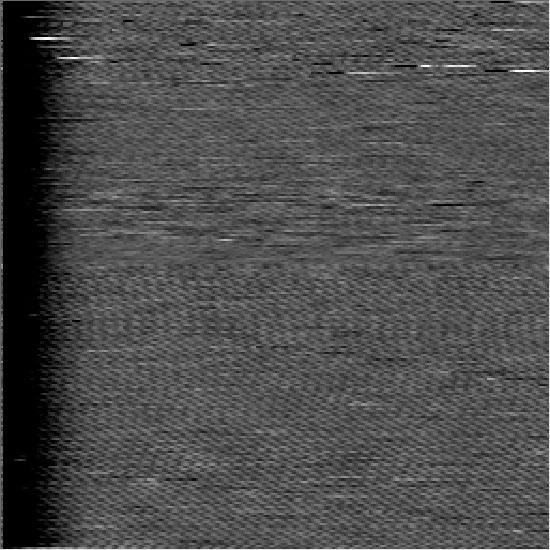
\includegraphics[width=.45\linewidth]{img/1550 - 调整增强.png}}
	\quad
	\subfloat[得到原子分辨图像]{\label{fig:firstTry-d}
		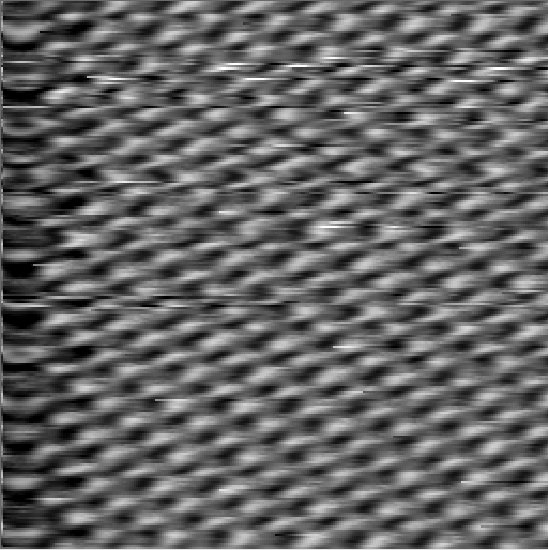
\includegraphics[width=.45\linewidth]{img/1647 - 原子分辨.png}}\\[2ex]
	\caption[初试]{石墨(\textup{HOPG})的\textup{STM}图像,
		参数如下表所示:\vspace{1.8ex}}
	\scriptsize
	\begin{tabularx}{.85\linewidth}{*9{C{1}}}
	\toprule\midrule
		\multirow{3}{*}{\hfil 图像} &
		\multicolumn{2}{c}{$V_x/\si{\V}$} &
		\multicolumn{2}{c}{$V_y/\si{\V}$} &
		\multirow{3}{*}{$I/\si{\nA}$} &
		\multirow{3}{*}{$V_\textup{b}/\si{\mV}$} &
		\multirow{3}{*}{$T/\si{\ms}$} &
		\multirow{3}{*}{\textup{Amp}} \\
		& 起点 & 范围 & 起点 & 范围 & & & & \\
		& ORIGIN & RANGE & ORIGIN & RANGE & & & & \\
	\midrule
		\ref{fig:firstTry-a} & 0 & 200 & 0 & 200 &
			1.13 & 1000 & 2000 & 20 \\
		\ref{fig:firstTry-b} & 190 & 10 & 100 & 10 &
			1.13 & 1000 & 300 & 50 \\
		\ref{fig:firstTry-c} & 190 & 10 & 100 & 10 &
			1.08 & 500 & 500 & 100 \\
		\ref{fig:firstTry-d} & 198 & 2.00 & 100 & 1.36 &
			1.08 & 500 & 350 & 100 \\
	\midrule\bottomrule
	\end{tabularx}
	\label{fig:firstTry}
	\end{figure}
\FloatBarrier
\subsection{原子分辨像}
	图 \ref{fig:firstTry-b} 的扫描范围已经较小,但此时图像的对比度依然很弱;因此,我们尝试在不改变扫描范围的前提下,通过增大Amp, $T$, 以及微调隧穿电流$I$, 从而获得更加清晰的图像。然而,实践表明,上述参数的调整对图 \ref{fig:firstTry-b} 像质的提升并不显著。这时,我们联想到了光学中的结论——可适当降低照明的亮度,即尝试在暗场条件下成像;对应于STM系统,调低“亮度”相当于减小偏压$V_\textup{b}$. 如此调整后,我们得到了如图 \ref{fig:firstTry-c} 所示的像,可见分辨度有显著提升。
	
	事实上,由于反馈电路的存在,上述光学类比并不完全成立;事实上,隧穿电流$I\sim\SI{1}{\nA}$基本不变,根据前面给出的式 \eqref{eq:tunnelEq}, 即:
	\begin{equation}
		I \sim B\,e^{-2\kappa s},\quad
		\kappa \sim \frac{\sqrt{2m\phi}}{\hbar},\quad
		B \sim I_0 \frac{16E}{\phi}
		\tag{\ref{eq:tunnelEq}}
	\end{equation}
	减小偏压$V_\textup{b}$, 导致系数$B$减小;反馈系统为了维持隧穿电流,将减小针尖与样品之间距$s$, 这才是像质提升的根本原因。在此基础上,进一步缩小扫描范围,最终得到了清晰的原子分辨像 \ref{fig:firstTry-d}. 
	
	\newparagraph
	理论上,只要观察到隧穿电流,便可视作量子隧穿效应的成功验证。然而,由于实验条件不尽完美,实际上总可以将十分微弱的隧穿电流归咎于实验系统的某种缺陷(\textit{例如,由于系统并非处于绝对的真空当中,可将电流解释为局部电离、尖端放电})。我们推测,这可能是历史上隧穿效应在很长一段时间内未被重视的一大原因(\textit{参见引言,隧穿效应很早便被实验观测到,却直到解释原子核衰变时才被人们重视})。
	
	因此,如图 \ref{fig:firstTry-d} 所示的原子分辨像是隧穿效应最强有力的\CJKunderdot{直观验证}。它直接反映了量子理论的有效性,并彻底消灭了历史上最后一小撮对\textit{原子的存在性}仍持怀疑态度的人\supercite{gamow2012one}。这也是本次实验中最为重要的结果。在图 \ref{fig:firstTry-d} 的基础上进一步减小扫描范围、微调参数,更为清晰的像如图 \ref{fig:imgRefined} 所示。
	
	\begin{figure}[p]
	\centering
	\vspace{-0.3\baselineskip}
	\subfloat[接近系统的分辨极限]{\label{fig:imgRefined-a}
		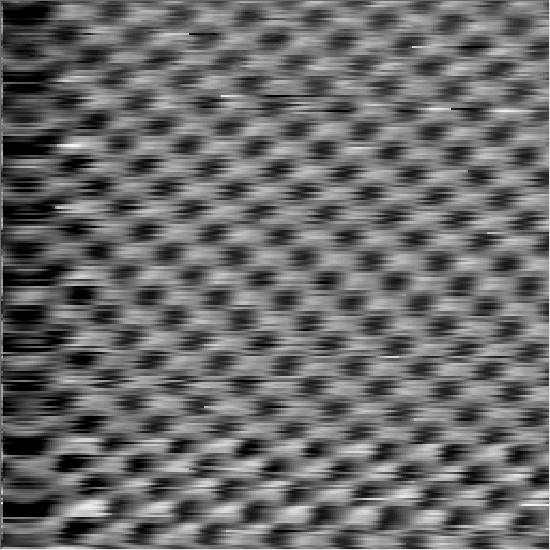
\includegraphics[width=.45\linewidth]{img/1711 - 极限分辨.png}}
	\quad
	\subfloat[\textup{\ref{fig:imgRefined-a}} 的对比度优化]{\label{fig:imgRefined-b}
		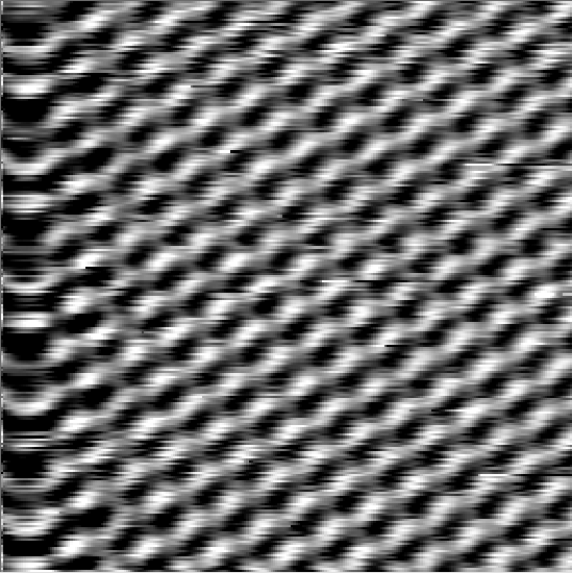
\includegraphics[width=.45\linewidth]{img/1800 - 对比增强.png}}\\
	\subfloat[进一步调整$x,y$比例后的结果]{\label{fig:imgRefined-c}
		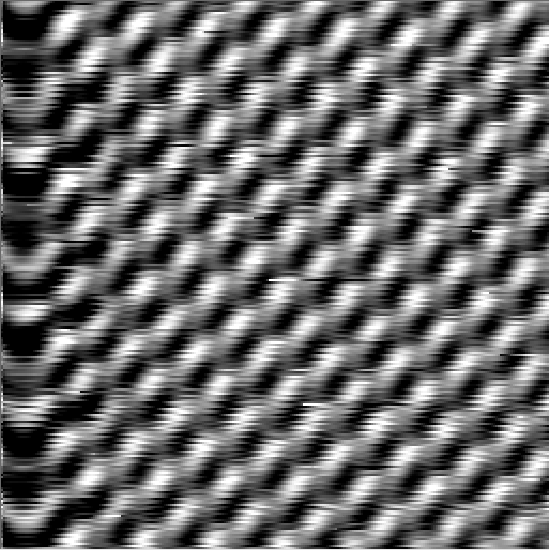
\includegraphics[width=.45\linewidth]{img/1835 - 比例调整.png}}\\[2ex]
	\caption[初试]{石墨(\textup{HOPG})的\textup{STM}图像,
		参数如下表所示:\vspace{1.8ex}}
	\scriptsize
	\begin{tabularx}{.85\linewidth}{*9{C{1}}}
	\toprule\midrule
		\multirow{3}{*}{\hfil 图像} &
		\multicolumn{2}{c}{$V_x/\si{\V}$} &
		\multicolumn{2}{c}{$V_y/\si{\V}$} &
		\multirow{3}{*}{$I/\si{\nA}$} &
		\multirow{3}{*}{$V_\textup{b}/\si{\mV}$} &
		\multirow{3}{*}{$T/\si{\ms}$} &
		\multirow{3}{*}{\textup{Amp}} \\
		& 起点 & 范围 & 起点 & 范围 & & & & \\
		& ORIGIN & RANGE & ORIGIN & RANGE & & & & \\
	\midrule
		\ref{fig:imgRefined-a} & 198 & 2.00 & 100 & 1.20 &
			1.08 & 500 & 250 & 100 \\
		\ref{fig:imgRefined-b} & 198 & 2.00 & 100 & 1.20 &
			1.08 & 250 & 250 & 100 \\
		\ref{fig:imgRefined-c} & 198 & 2.00 & 100 & 1.00 &
			1.03 & 250 & 250 & 100 \\
	\midrule\bottomrule
	\end{tabularx}
	\label{fig:imgRefined}
	\end{figure}
\subsection{图像分析}
	观察图像可见,白色斑点与黑色斑点间隔排列,两者各自均是\CJKunderdot{有心}的六角密排。这似乎与我们已知的HOPG结构,即\CJKunderdot{空心}的正六边形结构不太一致。
	
	事实上,如\autoref{fig:HOPGstruct} 所示,石墨表层的原子可分为两类:A类原子是上层原子正对着下层原子,两层原子的电子云($\pi$键)重合,导致A类原子的电子云趋于内部;B类原子则是上层原子正对下层空隙,其电子云更为自由,分布更广\supercite{LABUNIT530:online}。
	
	由于两类原子的电子云分布情况不同,根据STM的原理不难得出,两种原子在图像上表现出的“高度”不同;事实上,A, B类原子分别对应图像中的黑、白斑点;如果只看A或B类原子,自然是有心的六角密排。
	
	\begin{figure}[!h]
	\centering
	\vspace{-.5\baselineskip}
	\parbox{.45\linewidth}{
		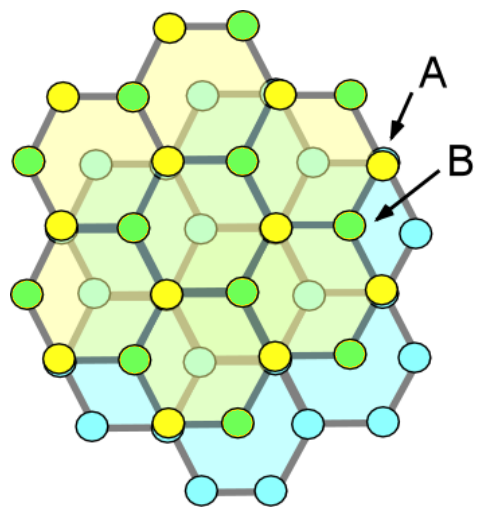
\includegraphics[width=\linewidth]{HOPGstruct.png}}\quad
	\parbox{.45\linewidth}{
		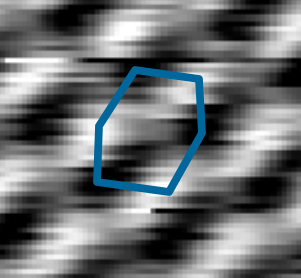
\includegraphics[width=\linewidth]{img/1800 - 对比增强 - MOD.png}}
	\caption[HOPG]{石墨(\textup{HOPG})的原子排列及
		单位正六边形在图 \textup{\ref{fig:imgRefined-b}} 中的体现,
		参见 \cite{LABUNIT530:online}. \\
		其中\textup{A}类原子正对下一层的原子,而\textup{B}类原子正对下一层中的“空洞”。\\
		图中黄色为表层\textup{A}类原子,绿色为表层\textup{B}类原子,蓝色为第二层原子。
		\vspace{.5ex}
	}
	\label{fig:HOPGstruct}
	\end{figure}
	
	\vspace{-3ex}
	由此,已知原子间隔为$a = \SI{2.46}{\angstrom}$, 我们可以粗略估计压电系数$c_{x,y}$. 仍然采用图 \ref{fig:imgRefined-b}, 利用线性关系 \eqref{eq:piezoEq}, 可得:
	\begin{equation}
		c_x \sim c_y \sim \SI{1}{\nm/\V}
	\end{equation}
	
	注意,上面给出的压电系数$c_{x,y}$仅仅是一个数量级估计;由图像 \ref{fig:imgRefined-b}, \ref{fig:imgRefined-c} 中正六边形网格的畸变不难看出,针尖显然不与样品表面垂直;同时,热漂移对成像的影响也比较显著,需要进一步研究。
\section{结论}
%%	首先要给出实验结果,然后再给出由实验结果分析得到的结果和结论.此部分给出的内容要比摘要中的全面,用词要更准确.\par
%%%%%%%%%%%%%%%%%%%%%%%%%%%%%%
	本实验对高定向热解石墨(HOPG)样品表面进行了STM扫描和测量,观察并得到了其原子级分辨像,并对像的结构进行了简单的解释。
	
	本实验所获得的原子分辨像是对隧穿效应乃至原子论的最强有力验证。这一技术突出了精准控制与精确测量的重要性,这也是实现该技术的主要困难;同时,STM的直观性也揭示了其巨大的潜能,预示着扫描探针显微技术将在科学研究和纳米加工技 术中发挥出越来越大的作用。
\section{致谢}
%	此部分感谢同组人...和对实验和报告有帮助的人.
%%%%%%%%%%%%%%%%%%%%%%%%%%%%%%
	能亲眼见到原子,不能不说是十分震撼的。感谢前人的努力,感谢科技的进步;感谢与我合作的邹瑜同学,他对像质的优化做出了巨大的贡献。感谢不错的运气(\textit{抑或是不错的人品?}),助我们获得了挺好的图像。当然,最感谢幽默而耐心的季航老师给我们带来的巨大帮助。

\setlength{\bibsep}{10pt}
\linespread{1.2}\selectfont
\bibliographystyle{../BibStyle/gbt-7714-2015-numerical}
\bibliography{../BibStyle/Textbook,bib/Ref}

\clearpage
\end{document}
